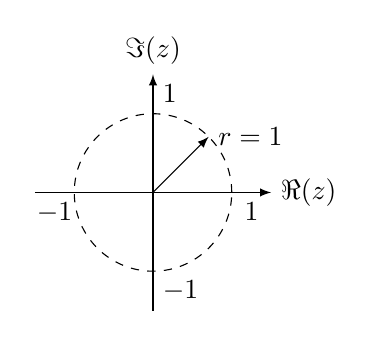
\begin{tikzpicture}[scale=1,>=latex]
        % draw the coordinates
        \draw[->] (-1.5cm,0cm) -- (1.5cm,0cm) node[right,fill=white] {$\Re(z)$};
        \draw[->] (0cm,-1.5cm) -- (0cm,1.5cm) node[above,fill=white] {$\Im(z)$};

        % draw the unit circle
        \draw[dashed] (0cm,0cm) circle(1cm);
        
        \draw[->] (0,0) -- (45:1) node[right] {$ r=1 $};

        % draw the horizontal and vertical coordinates
        % the placement is better this way
        \draw (-1.25cm,0cm) node[below] {$ -1 $}
              (1.25cm,0cm)  node[below] {$ 1 $}
              (0cm,-1.25cm) node[right] {$ -1 $}
              (0cm,1.25cm)  node[right] {$ 1 $};
    \end{tikzpicture}